\section{Introduction}
\label{sec:intro}

% The emergence of a new breed of computer
Embedded devices are growing impressively in popularity and ubiquity in recent years.
This growth can be attributed to the emergence of new application domains inspired by small, 
highly resource constrained programmable processors known as microcontroller units (or MCUs), 
some which can have as little of 2KB of RAM. It is now the case that less than 1 percent of 
the world's processors reside in general purpose computers such as desktop PCs, laptops and tablets 
- with MCUs picking up the remainder.
Furthermore, demand for MCUs continues to grow due to their use in the monitoring and 
controlling of a wide variety of systems, ranging from wearables, to home automation, to 
industrial automation and smart grids - a phenomenon broadly referred to as the Internet of Things (IoT).

MCUs are highly resource limited devices, but are not simply smaller versions of laptop and desktops. 
They are architecturally quite distinct. If we are to undertand how to optimize 
programming languages and their implementation for such devices it is worth dwelling on their key characteristics. 
Table \ref{table:devices} highlights the core capabilities of three state of the art devices vs. a typical PC. 

\begin{table}[]
    \centering
    \begin{tabular}{|l|r|r|r|r|r|}
    \hline
                           &          &              & \bf{Word}  &                 \\
    \bf{Device}            & \bf{RAM} & \bf{Flash}   & \bf{Size}  & \bf{CPU Speed}  \\ \hline
    Arduino Uno            & 2 KB       & 32 KB      & 8          & 16MHz AVR       \\ \hline
    BBC micro:bit          & 16 KB      & 256 KB     & 32         & 16MHz nRF51     \\ \hline
    Adafruit CPX           & 32 KB      & 256 KB     & 32         & 48MHz SAM    \\ \hline
    Typical PC             & 16 GB      & 1 TB       & 64         & 3GHz Intel      \\ \hline
    \end{tabular}
    \caption{\label{table:devices}Example microcontroller devices in relationship to a typical PC (SAM = SAMD21).}
    \end{table}

While it is clear that all such devices are highly resource contrained compared to modern PCs 
(about six orders of magnitude on most metrics), a deeper analysis derive two further key observations.

Firstly, \emph{MCUs are processor rich}. Contrary to popular belief, these devices have 
a \emph{proportionally} large amount of processing power. For example - consider the BBC micro:bit 
versus a typical PC. It has about 100 times less CPU power, but 10\textsuperscript{6} times less RAM, 
and 10\textsuperscript{6} time less storage. A good programming language design should therefore not 
only \emph{seek to provide high code density and spatial efficiency, 
but to actively trade off CPU for spatial efficiency where possible}. 

Secondly, \emph{MCUs are accumulating more features on chip}. 
MCUs still follow Moore's law (the number of transistors doubles roughly every two years). 
However, this additional capacity is 
not typically invested in simply optimizing processing power. Instead, \emph{independent peripherals} 
are integrated onto the same silicon chip as the CPU. Examples include integrated radio hardware such 
as Bluetooth/WiFi and audio inputs and outputs. This hardware is designed to run independently of the 
CPU, hence \emph{an effective application programming language should directly support such an asynchronous
interaction model}.

% Despite this languages and programming environments have yet to keep pace with the mainstream (e.g. Arduino/mbed)
Furthermore, with this surge in the demand for MCUs across a wide spectrum of applications, 
there is a need to simplify the programming of such devices so that more people can participate in 
the creation of MCU-based systems. From rapid product innovation to education,
we have seen a sustained growth in the volume and diversity of people wishing to program MCU-based devices.
% JOE: do we have a citation??? 

These new application developers share a common characterisitic - \emph{they are not professional software developers}. 
Programming languages and development environments for MCUs have not kept pace with these advances 
in hardware and diversification of user domains. Elsewhere, we have long supported inexperienced developers through  
modern high level text-based languages for application development such as Java, C\#, Python and Javascript, and also 
through visual programming languages based on frameworks such as Blockly. 

In the world of the MCU, the C/C++ languages remain the standard, and for good reason. 
They provide a familiar imperative programming model, with compilers that produce highly efficient code (in terms of both 
temporal and spatial complexity), and enable low level access to hardware features when necessary. Examples
of this are commonplace, such as the Arduino project (\url{www.arduino.cc})~\cite{buildingArduino2014},
started in 2003, and the ARM mbed platform (\url{www.mbed.org})~\cite{ARMmbed} - both of which rely heavily on
a C/C++ programming model. However, the limitations of using C/C++ as an applicaiton programming language for 
inexperienced developers are well understood. 
% Doesn't feel like we really need to spell out the limitation of C/C++ out here. Anyone got good references?

% Paper overview
In this paper we introduce a novel architecture for MCU-based devices,
that is designed with three goals in mind: 
(1) it should be usable by \emph{anyone}, not just trained professionals; 
(2) it should be available \emph{anywhere}, requiring no specialized software (native applications
or device drivers) to operate;
(3) it should run efficiently on \emph{anything}, from devices with as little as 2KB of memory.
More specifically, we present and evaluate a platform that bridges the worlds of the web and the 
MCU through three novel technologies:

\begin{itemize}
\item \emph{Static TypeScript} is a statically-typed subset of TypeScript
(\url{www.typescriptlang.org}) that we have defined for fast execution on low-memory devices,
with a simple model for linking against pre-compiled C++ (Section~\ref{sec:sts});

\item \emph{\CO}, a component-based, event-driven, multi-threaded, C++ runtime environment
that bridges the semantic gap between higher-level languages (such as TypeScript) and the hardware,
modelling each hardware component as a software component (Section~\ref{sec:codal});

\item \emph{\MCN}, a web application containing an \emph{in-browser compiler} that supports the 
simplified programming of MCUs via editors for visual blocks and textual Javascript languages 
(Section~\ref{sec:makecode});
\end{itemize}

Our results show that these technologies combined can enable simplified programming through modern
languages and event based constructs while maintaining a relatively high degree of temporal and spatial efficiency. 
We show up to 50x more performant than other state-of-the-art implementations, 
in some cases nearing the performance of native C++. 

% Additional fodder we could work in if needed....
%even the most conservative estimates predict in excess of 
%30 billion IoT devices will be interconnected by 2020 [] - far outstripping the 3.7 billion people 
%and 1.2 billion websites using the internet today.


% The \MC \CO Architecture
    


\subsection{Architecture}



% Derive some key goals/requirements



% Include example app to architecture section


% Lacking context - broad statements could also be misinterpreted.
\begin{comment}
Web-based visual editors such as
Blockly (\url{https://developers.google.com/blockly/})~\cite{Blocky2015}
are tremendously popular and allow the creation of programs without the
possibility of syntax errors, and that execute in the web browser (Blockly
is written in JavaScript and compiles user code to JavaScript).
However, JavaScript's dynamic nature is not well-suited to the world of
MCUs where memory is limited (consider the Arduino Uno mentioned above).
\end{comment}

\begin{figure}[t]
    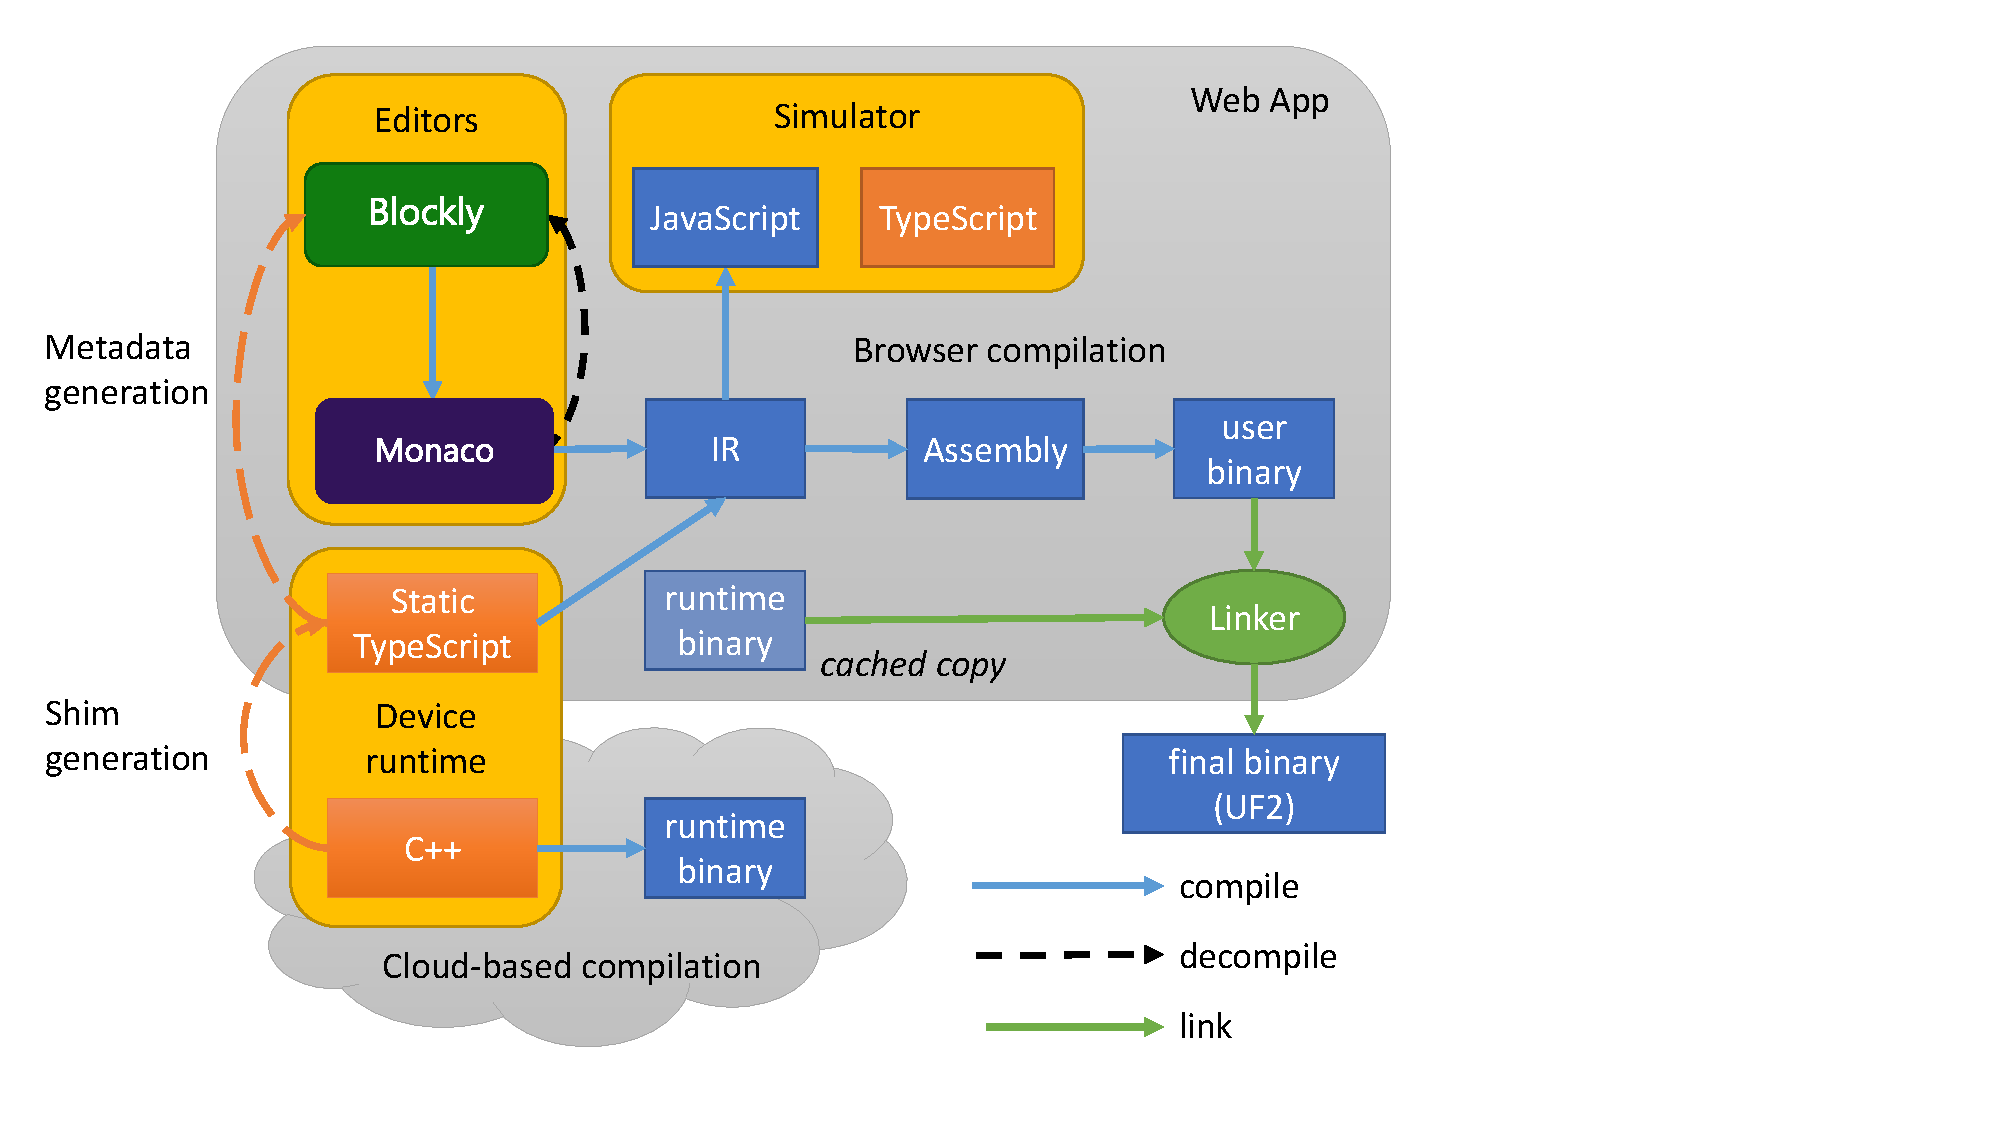
\includegraphics[width=4.8in]{makecodeFig.pdf}
\caption{\label{fig:makecode}\MC web app}
\end{figure}

% need to derive some key goals/requirements before here?
Figure~\ref{fig:makecode} shows a high-level architecture of
the \MC web app, the entry point of the platform that
incorporates the Blockly
(\emph{\href{https://github.com/google/blockly}{blockly}}) and Monaco
(\emph{\href{https://github.com/Microsoft/monaco-editor}{monaco-editor}}
editors (upper-left), in-browser execution via a device simulator (upper-right),
as well as compilation of Static TypeScript to machine code and linking against 
the C++ runtime (\emph{\CON}), pre-compiled by a cloud service (lower-left).

The statically-typed runtime and type inference on user code allows uses to write code
that looks like plain JavaScript (see Figure~\ref{fig:example}) and progress later to working
with types. As can be seen im Figure~\ref{fig:makecode}, 
no C/C++ compiler is needed to compile the Static TypeScript user code (coming from Monaco);
the result of compilation is a binary file that is ``downloaded'' from the web app to the user's
computer and then flashed to the MCU (exposed as a USB pen drive)
via a simple file copy operation.

These advances enable beginners to get started programming MCUs from
any modern web browser, and enable hardware vendors to innovate and safely add new
components to the mix using Static TypeScript.
Once the web app has been loaded, all the above functionality works offline
(i.e., if the host machine loses its connection
to the internet). All of the platform's components are open source on GitHub.

Table~\ref{table:devices} lists a number of the devices/MCUs supported by our platform,
ranging from the highly resource-contrained Arduino Uno to the slightly less constrained space of
the micro:bit, and Adafruit Circuit Playground Express (CPX).

\subsection{Running Example: firefly simulation.}

Figure~\ref{fig:example} shows a JavaScript
program that implements a simple ``firefly'' example
for the Adafruit Circuit Playground Express (CPX).
This program demonstrates the natural phenomenon
of fireflies synchronizing their light pulses (the program should be
run on several CPX's close to each other in a dark room).

The program has three top-level statements:
the first initializes the global variable \emph{clock} (line 1); the
second registers an event handler (a lambda function) to execute
each time the CPX's light detector senses a bright light (line 3); the
third registers a lambda function to run forever on a fiber (line 18),
to keep track of time and pulse the CPX's 10 LEDs whenever the
clock reaches 8.

Note that this program is a JavaScript program, as there are no
types mentioned explicitly. However, all the functions called in
this program are part of the runtime and are explicitly
typed. This program is a Static TypeScript program:
the static type of every variable and expression
can be inferred and passes the more restrictive checks
of Static TypeScript, as detailed in Section~\ref{sec:sts}.

The program also shows off the use of the non-preemptive concurrency
model supported by both \MC (for JavaScript) and \CO (for C++).
The forever procedure executes the lambda inside a ``while (true)''
loop that yields (via a call to \emph{basic.pause}) after each call to the lambda.
This gives the light-detection event handler a chance to execute
upon user input (in a separate fiber). Although the global variable \emph{clock} is
shared by the two fibers, there is no data race due to the non-preemptive
scheduling model.

\begin{figure}
\begin{lstlisting}
  let clock = 0

  input.onLightConditionChanged(
    LightCondition.Bright, () => {
      if (clock < 8) {
          clock += 1    // catchup to neighbor
      }
  })

  loops.forever(() => {
    if (clock >= 8) {
        // notify neighbors
        light.setAll(Colors.White)
        loops.pause(200)
        light.clear()
        clock = 0         // reset the clock
    } else {
        loops.pause(100)
        clock += 1
    }
})
\end{lstlisting}
\caption{\label{fig:example}Running example: firefly simulation.}
\end{figure}

\subsection{Overview}
Sections~\ref{sec:makecode} to~\ref{sec:codal} presents the three major components of the platform:
\MC, Static TypeScript, and \CO. Section~\ref{sec:evaluate} evaluates the performance of the platform,
Section~\ref{sec:related} discusses related work, and Section~\ref{sec:conclude}
concludes.